% Copyright (C) 2017 - J Schueller

\documentclass{beamer}



%\setbeameroption{hide notes}
%\setbeameroption{show notes}
%\setbeameroption{show only notes}

  % Copyright (C) 2012 - EDF R&D - Michael Baudin

% To highlight source code
\usepackage{listings}
\definecolor{darkgreen}{rgb}{0,0.5,0}
\definecolor{violet}{rgb}{0.5,0,1}

\usepackage{lmodern}% http://ctan.org/pkg/lm

\usetheme{Montpellier}
\setbeamertemplate{navigation symbols}{} % Remove navigation
\useoutertheme{infolines}

\usepackage[utf8]{inputenc}
\usepackage[T1]{fontenc}

%\usepackage[french]{babel}
%\uselanguage{French}
%\languagepath{French}

\def\bx{{\bf x}}
\def\RR{\mathbb{R}}

\newcommand{\pyvar}[1]{\texttt{#1}}

\def \ot {OpenTURNS}

\hypersetup{colorlinks=true}

\usepackage{adjustbox}


\title[Low rank tensor approximation]{
Low rank tensor approximation in OpenTURNS
}

\author[J. Schueller]{\textbf{J. Schueller}}

\institute[Phimeca]{Phimeca}

\vspace*{-1.0cm}
\date[]{\\CHORUS workshop, 2017-10-19}

%%%%%%%%%%%%%%%%%%%%%%%%%%%%%%%%%%%%%%%%%%%%%%%%%%%%%%%%%%%%%%%%%%%%%%%%%%%%%

\begin{document}

%------------------------------------------------------------------------------------------------------
\part{TITLEPAGE}
%------------------------------------------------------------------------------------------------------
\begin{frame}
  \titlepage
  \vspace*{-1cm}
  \hspace*{5cm}
  \begin{figure}[b]
    \hspace*{0.5cm}
%     \vspace*{-1.0cm}
%     \vspace*{1.0cm}
    %\logophimeca{scale=.05}\phimeca
    %\hspace*{6.0cm}
    
    \raisebox{4mm}{\begin{minipage}{1cm}
      {
\includegraphics[scale=.15]{figures/icon256.png}}
    \end{minipage}}
  \end{figure}
\end{frame}

% \scriptsize
%------------------------------------------------------------------------------------------------------
\part{INTRODUCTION}
% Pas de niveau section -> on passe direct en subsection pour ne pas alourdir les cadres en haut avec le plan à va venir
%------------------------------------------------------------------------------------------------------

% \subsection[Contexte et objectifs]{Contexte et objectifs}
% \begin{frame}
%   \frametitle{Contexte et objectifs}
%   \begin{block}{Contexte}
%    \begin{itemize}
%     \item Point 1
%     \item Point 2
%     \item Point 3
%    \end{itemize}
%   \end{block}
%   \begin{block}{Objectifs}
%    \begin{enumerate}
%     \item Point 1
%     \item Point 2
%     \item Point 3
%    \end{enumerate}
%   \end{block}
% \end{frame}

%------------------------------------------------------------------------------------------------------
\part{CONTENT}
%------------------------------------------------------------------------------------------------------

%------------------------------------------------------------------------------------------------------
% Plan general
%------------------------------------------------------------------------------------------------------

\begin{frame}
  \frametitle{Plan}
  \begin{columns}
  \begin{column}{0.1 \textwidth}\end{column}
  \begin{column}{0.9 \textwidth}
  \tableofcontents[part=3,hideallsubsections]%,pausesections]
  \end{column}
  \end{columns}
\end{frame}


% from __future__ import print_function
% import openturns as ot
% from math import pi
% from openturns.viewer import View
% 
% #factory = ot.FourierSeriesFactory(); xmin=-pi; xmax=pi
% factory = ot.HaarWaveletFactory(); xmin=0.0; xmax=1.0
% 
% #print(factory)
% x = 0.4
% ag=ot.Graph()
% for i in range(5):
%     f = factory.build(i)
%     g= f.draw(xmin, xmax, 100)
%     d=g.getDrawable(0)
%     d.setLegend('Haar '+str(i))
%     ag.add(d)
% ag.setDefaultColors()
% print(ot.Graph.GetValidLegendPositions())
% ag.setLegendPosition('bottomright')
% ot.Show(ag)
% #View(ag).save('haar.png')
% View(ag).save('haar.png')

%------------------------------------------------------------------------------------------------------
\section[Non-polynomial basis]{Non-polynomial basis}
%------------------------------------------------------------------------------------------------------

\subsection[Fourier series]{Fourier series}
\begin{frame}
  \frametitle{Fourier series}
  \begin{block}{Fourier series}
    $$
    \begin{array}{lcl}
      \psi_0(x)      & = & 1 \\
      \psi_{2k+1}(x) & = & \sqrt{2}\sin(kx) \\
      \psi_{2k+2}(x) & = & \sqrt{2}\cos(kx)
    \end{array}
    $$
  \end{block}
  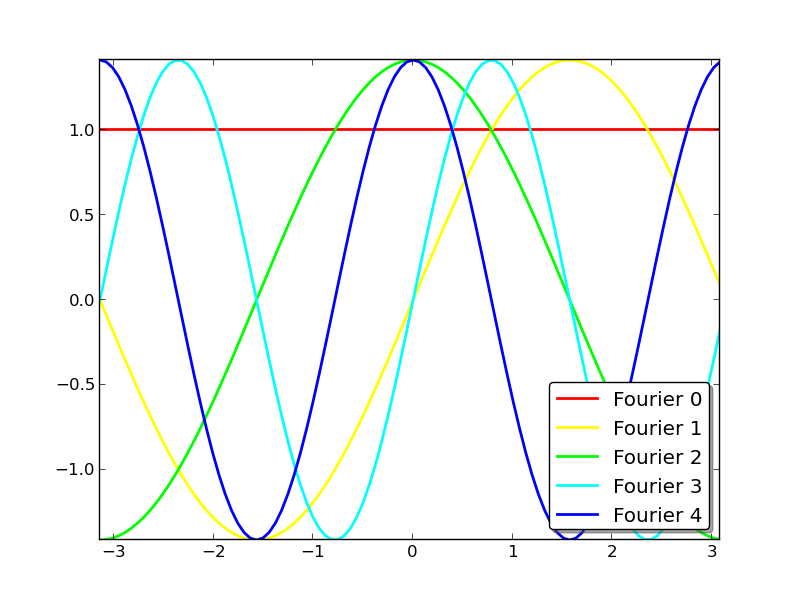
\includegraphics[scale=0.3]{figures/fourier.png}
\end{frame}

\subsection[Haar wavelets]{Haar wavelets}
\begin{frame}
  \frametitle{Haar wavelets}

  \begin{block}{Haar wavelets}
    $$
    \begin{array}{lcl}
      \psi_0(x) & = & \fcar{[0, 1]}{x} \\
      \psi_n(x) & = & \frac{1}{2^{j/2}}\left[\fcar{[\frac{k}{2^j},\frac{k+1/2}{2^j}]}{x}-\fcar{[\frac{k+1/2}{2^j},\frac{k+1}{2^j}]}{x}\right]
    \end{array}
    $$
  \end{block}
  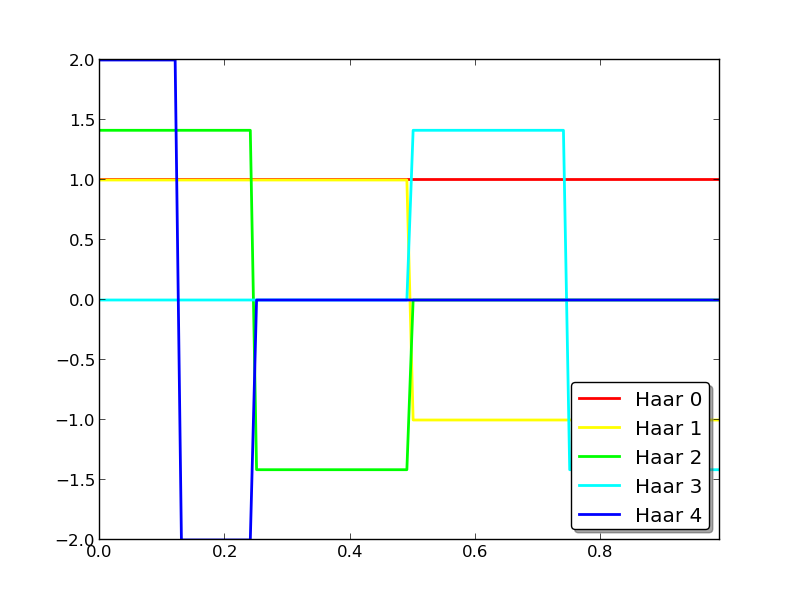
\includegraphics[scale=0.3]{figures/haar.png}
\end{frame}

% \subsection[Basis usage]{Basis usage}
\begin{frame}[containsverbatim]
  \frametitle{Usage}
  \begin{block}{In Python...}
    \begin{lstlisting}
    # as a regular function
    family = ot.FourierSeriesFactory()
    family = ot.HaarWaveletFactory()

    for i in range(5):
        f = family.build(i)
        d = f.draw(xmin, xmax, 100)
    \end{lstlisting}
  \end{block}
\end{frame}

\subsection[Tensorization]{Tensorization}
\begin{frame}
  \frametitle{Functional chaos tensorization}
  \begin{block}{Tensorization}
    Functional chaos decomposition
    $$
    Y \, \,  \equiv \, \,  h(\underline{X}) \, \, = \, \, \sum_{j=0}^{\infty} \; a_{j} \; \psi_{j}(\underline{X})
    $$
    on univariate orthogonal function families
    $$
    \phi^{(j)}_1, ..., \phi^{(j)}_M ~~~~~ \forall j \in [1, d]
    $$
    upon tensorized basis
    $$
    \psi_{\idx}(\vect{x}) \, \, \equiv \,\, \phi^{(1)}_{\alpha_{1}}(x_{1}) \times \cdots \times \phi^{(d)}_{\alpha_{d}}(x_{d})
    $$
  \end{block}
\end{frame}



\begin{frame}
  \frametitle{Functional chaos tensorization}
  \begin{block}{Tensorization}
    upon tensorized basis
    $$
    \psi_{\idx}(\vect{x}) \, \, \equiv \,\, \phi^{(1)}_{\alpha_{1}}(x_{1}) \times \cdots \times \phi^{(d)}_{\alpha_{d}}(x_{d})
    $$
    multi-indices notation
    $$
    \alpha \equiv \{\alpha_{1},\dots,\alpha_{d}\}
    $$
    curse of dimensionality
    $$
    P = C^{d+M}_{M}
    $$
  \end{block}
  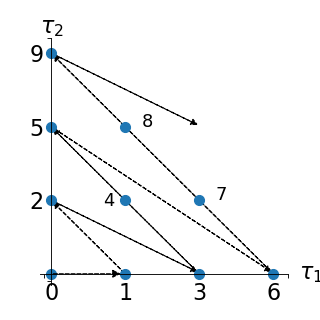
\includegraphics[scale=0.3]{figures/enumerate.png}
\end{frame}



% \subsection[Tensorization]{Tensorization}
\begin{frame}[containsverbatim]
  \frametitle{Usage}
  \begin{block}{In Python...}
    \begin{lstlisting}

    # polynomial basis
    ef = ot.LinearEnumerateFunction(dim)
    factC = [LegendreFactory()] * dim
    prod = ot.OrthogonalProductPolynomialFactory(factC, ef)

    # non-polynomial basis
    factC = [ot.FourierSeriesFactory()] * dim
    prod = ot.OrthogonalProductFunctionFactory(factC)

    algo = ot.FunctionalChaosAlgorithm(...)
    \end{lstlisting}
  \end{block}
\end{frame}

%------------------------------------------------------------------------------------------------------
\section[Canonical tensor]{Canonical tensor}
%------------------------------------------------------------------------------------------------------

\subsection[Canonical tensor]{Canonical tensor}
\begin{frame}
  \frametitle{Rank one tensor}
  \begin{block}{Rank one tensor}
  $$
  f(x_1, \dots, x_d) = \prod_{i=1}^d v_i (x_i)
  $$
  with
  $$
  v_i = \sum_{j=1}^{n_i} \alpha_j^{(i)} \phi_j(x_i)
  $$
  expanding to
  \begin{align*}
  f(x_1, \dots, x_d) & = (\alpha_1^{(1)} \phi_1(x_1)+\dots+\alpha_{n_1}^{(1)} \phi_{n_1}(x_1)) \\
                & \times \dots \\
                & \times (\alpha_1^{(d)} \phi_1(x_d)+\dots+\alpha_{n_d}^{(d)} \phi_{n_d}(x_d))
  \end{align*}

  \end{block}

\end{frame}


\begin{frame}

  \begin{block}{Canonical tensor format}
  Available representation
  $$
  f(x_1, \dots, x_d) = \sum_{k=1}^r \prod_{i=1}^d v_i^{(k)} (x_i)
  $$
  with
  $$
  v_i = \sum_{j=1}^{n_i^{(k)}} \alpha_j^{(i,k)} \phi_j(x_i)
  $$
  linear number of terms wrt dimension
  $$
  P = r \sum_{i=1}^d n_i
  $$
  \end{block}

\end{frame}


\subsection[Algorithms]{Algorithms}
\begin{frame}[fragile]
  \frametitle{Alternating Least Squares}
  \begin{block}{Alternating Least Squares algorithm}

Allows to learn a rank-one tensor.
\begin{algorithm}[H]
\begin{algorithmic}[1]
\STATE Initialize $v_i(x_i) = 1$
\WHILE{$v$ does not converge}
\FOR{$i=1$ to $d$}
\STATE [$\Psi^i(x)]_j = \prod_{u=1 \neq i}^d v_u (x_u) \phi_j^i(x_i) $
\STATE Solve $\underset{\beta_i}{\operatorname{argmin}} ||y - \Psi^i(x) ^t \beta_i ||_2^2$
\ENDFOR
\ENDWHILE
\end{algorithmic}
\caption{ALS}
\label{alg:seq1}
\end{algorithm}

\end{block}
\end{frame}

\begin{frame}[fragile]
  \frametitle{Greedy rank-one approximation}
  \begin{block}{Alternating Least Squares algorithm}

Allows to learn a rank-r tensor.
\begin{algorithm}[H]
\begin{algorithmic}[1]
\STATE Rank-1 approximation $\prod_{i=1}^d v_i^{(1)} (x_i)$
\FOR{$r=2$ to $r_{max}$}
\STATE Rank-1 approximation $\prod_{i=1}^d v_i^{(r)} (x_i)$
\STATE $y^m = y - \sum_{k=1}^r \alpha_k \prod_{i=1}^d v_i^{(r)} (x_i)$
\STATE Update $\alpha$ to minimize error (least-squares)
\ENDFOR
\end{algorithmic}
\caption{Greedy rank-one}
\label{alg:seq}
\end{algorithm}

\end{block}
\end{frame}


\begin{frame}[containsverbatim]
  \frametitle{Usage}
  \begin{block}{In Python...}
\begin{lstlisting}
import openturns as ot

def model(X):
    ...
    return Y

r = 4
dim = 5
nk = [10] * dim
factC = [ot.FourierSeriesFactory()] * dim
prod = ot.OrthogonalProductFunctionFactory(factC)
X = dist.getSample(size)
Y = model(X)
algo = ot.TensorApproximationAlgorithm(X, Y, dist, factC, nk, r)
\end{lstlisting}
  \end{block}
\end{frame}

% 
% \subsection[Screening]{Screening}
% \begin{frame}
%   \frametitle{P0 Failures}
%   Among failure samples, P0 CDF is non-linear below $2.10^{-4}$
%   \includegraphics[scale=0.4]{P0_cdf.png}
% \end{frame}
% 
% \subsection[Screening]{Screening}
% \begin{frame}
%   \frametitle{X2 Failures}
%   New design experiment, P0>$2.10^{-4}$, N=5000, 41h/1cpu, 93 failures.
%   \includegraphics[scale=0.3]{pm_X2.png}
% \end{frame}
% 
% \subsection[Screening]{Screening}
% \begin{frame}
%   \frametitle{X2 Failures}
%   Among failure samples, X2 CDF is non-linear below $0.08$
%   \includegraphics[scale=0.4]{X2_cdf.png}
% \end{frame}


% 
% 
% %------------------------------------------------------------------------------------------------------
% \section[Section 2]{Section 2}
% %------------------------------------------------------------------------------------------------------
% 
% \subsection[Sous section 1]{Sous section 1}
% \begin{frame}
%   \frametitle{Titre du transparent}
%   \framesubtitle{Sous-titre du transparent}
%   \begin{block}{Bloc 1}
%    \begin{itemize}
%     \item Point 1
%     \item Point 2
%     \item Point 3
%    \end{itemize}
%   \end{block}
%   \begin{block}{Bloc 2}
%    \begin{equation*}
%     y = a\,x + b
%    \end{equation*}
%   \end{block}
% \end{frame}
% 
% \subsection[Sous section 2]{Sous section 2}
% \begin{frame}
%   \frametitle{Titre du transparent}
%   \begin{columns}
%     \begin{column}{.5\textwidth}
%       \begin{block}{Bloc 1}
%       \begin{itemize}
%   \item Point 1
%   \item Point 2
%   \item Point 3
%       \end{itemize}
%       \end{block}
%     \end{column}
%     \begin{column}{.5\textwidth}
%       \begin{block}{Bloc 2}
%   \begin{equation*}
%     y = a\,x + b
%   \end{equation*}
%       \end{block}
%     \end{column}
%   \end{columns}
% \end{frame}
% 
% \subsection[Sous section 3]{Sous section 3}
% \begin{frame}
%   \frametitle{Titre du transparent}
%   \framesubtitle{Sous-titre du transparent}
%   \begin{itemize}
%     \item Point 1
%     \begin{itemize}
%       \item Point 1.1
%       \item Point 2.1
%       \item Point 3.1
%     \end{itemize}
%     \item Point 2 (une équation non numérotée)
%     \begin{equation*}
%       y = a\,x + b
%     \end{equation*}
%   \end{itemize}
% \end{frame}
% 
% \subsection[Sous section 4]{Sous section 4}
% \begin{frame}
%   \frametitle{Titre du transparent}
%   \framesubtitle{Sous-titre du transparent}
%   \begin{itemize}
%     \item Point 1
%     \begin{itemize}
%       \item Point 1.1
%       \item Point 2.1
%       \item Point 3.1
%     \end{itemize}
%     \item Point 2 (une équation non numérotée)
%     \begin{equation*}
%       y = a\,x + b
%     \end{equation*}
%   \end{itemize}
% \end{frame}
% 
% %------------------------------------------------------------------------------------------------------
% \section[Section 3]{Section 3}
% %------------------------------------------------------------------------------------------------------
% 
% \subsection[Sous section 1]{Sous section 1}
% \begin{frame}
%   \frametitle{Titre du transparent}
%   \framesubtitle{Sous-titre du transparent}
%   \begin{block}{Bloc 1}
%    \begin{itemize}
%     \item Point 1
%     \item Point 2
%     \item Point 3
%    \end{itemize}
%   \end{block}
%   \begin{block}{Bloc 2}
%    \begin{equation*}
%     y = a\,x + b
%    \end{equation*}
%   \end{block}
% \end{frame}
% 
% \subsection[Sous section 2]{Sous section 2}
% \begin{frame}
%   \frametitle{Titre du transparent}
%   \framesubtitle{Sous-titre du transparent}
%   \begin{block}{Bloc 1}
%    \begin{itemize}
%     \item Point 1
%     \item Point 2
%     \item Point 3
%    \end{itemize}
%   \end{block}
%   \begin{block}{Bloc 2}
%    \begin{equation*}
%     y = a\,x + b
%    \end{equation*}
%   \end{block}
% \end{frame}

%------------------------------------------------------------------------------------------------------
\part{CONCLUSION}
% Pas de niveau section -> on passe direct en subsection pour ne pas alourdir les cadres en haut avec le plan à va venir
%------------------------------------------------------------------------------------------------------

\subsection[Conclusion]{Conclusion}
\begin{frame}
  \frametitle{Conclusion}
  \begin{block}{Conclusions}
    \begin{enumerate}
      \item Greedy rank-1
      \item Regularized greedy rank-one
    \end{enumerate}
    \end{block}
    \begin{block}{Perspectives}
    \begin{itemize}
      \item Rank-M
%       \item Point 2
%       \item Point 3
    \end{itemize}
  \end{block}
\end{frame}

\end{document}